%%%%%%%%%%%%%%%%%%%%%%%%%%%%%%%%%%%%%%%%%%%%%%%%%%%%%%%
% A template for Wiley article submissions.
% Developed by Overleaf. 
%
% Please note that whilst this template provides a 
% preview of the typeset manuscript for submission, it 
% will not necessarily be the final publication layout.
%
% Usage notes:
% The "blind" option will make anonymous all author, affiliation, correspondence and funding information.
% Use "num-refs" option for numerical citation and references style.
% Use "alpha-refs" option for author-year citation and references style.

\documentclass[alpha-refs]{wiley-article}
% \documentclass[blind,num-refs]{wiley-article}

% Add additional packages here if required
\usepackage{siunitx}
\usepackage{lineno}

% Update article type if known
\papertype{Original Article}
% Include section in journal if known, otherwise delete
\paperfield{Pest Management Science}

\title{Spinosad baited spheres to attract and kill onion maggot (\textit{Delia antiqua})}

% List abbreviations here, if any. Please note that it is preferred that abbreviations be defined at the first instance they appear in the text, rather than creating an abbreviations list.
%\abbrevs{ABC, a black cat; DEF, doesn't ever fret; GHI, goes home immediately.}

% Include full author names and degrees, when required by the journal.
% Use the \authfn to add symbols for additional footnotes and present addresses, if any. Usually start with 1 for notes about author contributions; then continuing with 2 etc if any author has a different present address.
\author[1\authfn{1}]{Denis S. Willett}
\author[1\authfn{1}]{Camila C. Filgueiras}
\author[2]{Starker Wright}
\author[1]{Jan P. Nyrop}
\author[1]{Brian A. Nault}

\contrib[\authfn{1}]{Equally contributing authors.}

% Include full affiliation details for all authors
\affil[1]{Department of Entomology, Cornell AgriTech, Cornell University, Geneva, NY, 14456, USA}
\affil[2]{Bartlett Tree Experts, Dublin, PA, USA}

\corraddress{Denis S. Willett, 15 Castle Creek Drive, Geneva, NY 14456}
\corremail{deniswillett@cornell.edu}


% Include the name of the author that should appear in the running header
\runningauthor{Willett et al.}

\begin{document}

\maketitle

\begin{abstract}

% Please include a maximum of seven keywords
\keywords{Onion Maggot, \textit{Delia antiqua}, attraction, sticky-trap, attract-and-kill, lure, onion management}
\end{abstract}

\linenumbers
\section{Introduction}
\section{Materials and Methods}

Field trials evaluating the efficacy of attract and kill strategies to manage onion maggot populations were conducted from 2006 to 2008 in commercial dry bulb onion fields on muck soils in upstate New York.  Muck soils are high organic matter soils formed from old lake beds.  Trials were conducted from May to September.  

\subsection{Population Monitoring}

Population monitoring of onion maggot adults was accomplished by deploying white sticky cards with six replications in experimental plots.  Cards were collected weekly and the number of males and females counted.  

\subsection{Onion Maggot Mortality}

The ability of spinosad spheres to kill onion maggot flies was

\subsection{Field Damage}


\subsection{Analysis}
\subsection{Data Management}


\section{Results}

\paragraph{Population Monitoring}

\paragraph{Onion Maggot Mortality}

\paragraph{Field Damage}



\begin{figure}[bt]
\centering
\includegraphics[width = 8cm]{figures/final-figures/figure-1.pdf}
\caption{Population dynamics of adult onion maggot (\textit{D. antiqua} flies in upstate New York muck regions.  Points indicate observations of numbers of adult flies captured on sticky cards.  Lines and shaded regions indicate smoothed fits and 95\% confidence intervals respectively.  }
\label{fig:figure1}
\end{figure}

\begin{figure}[bt]
\centering
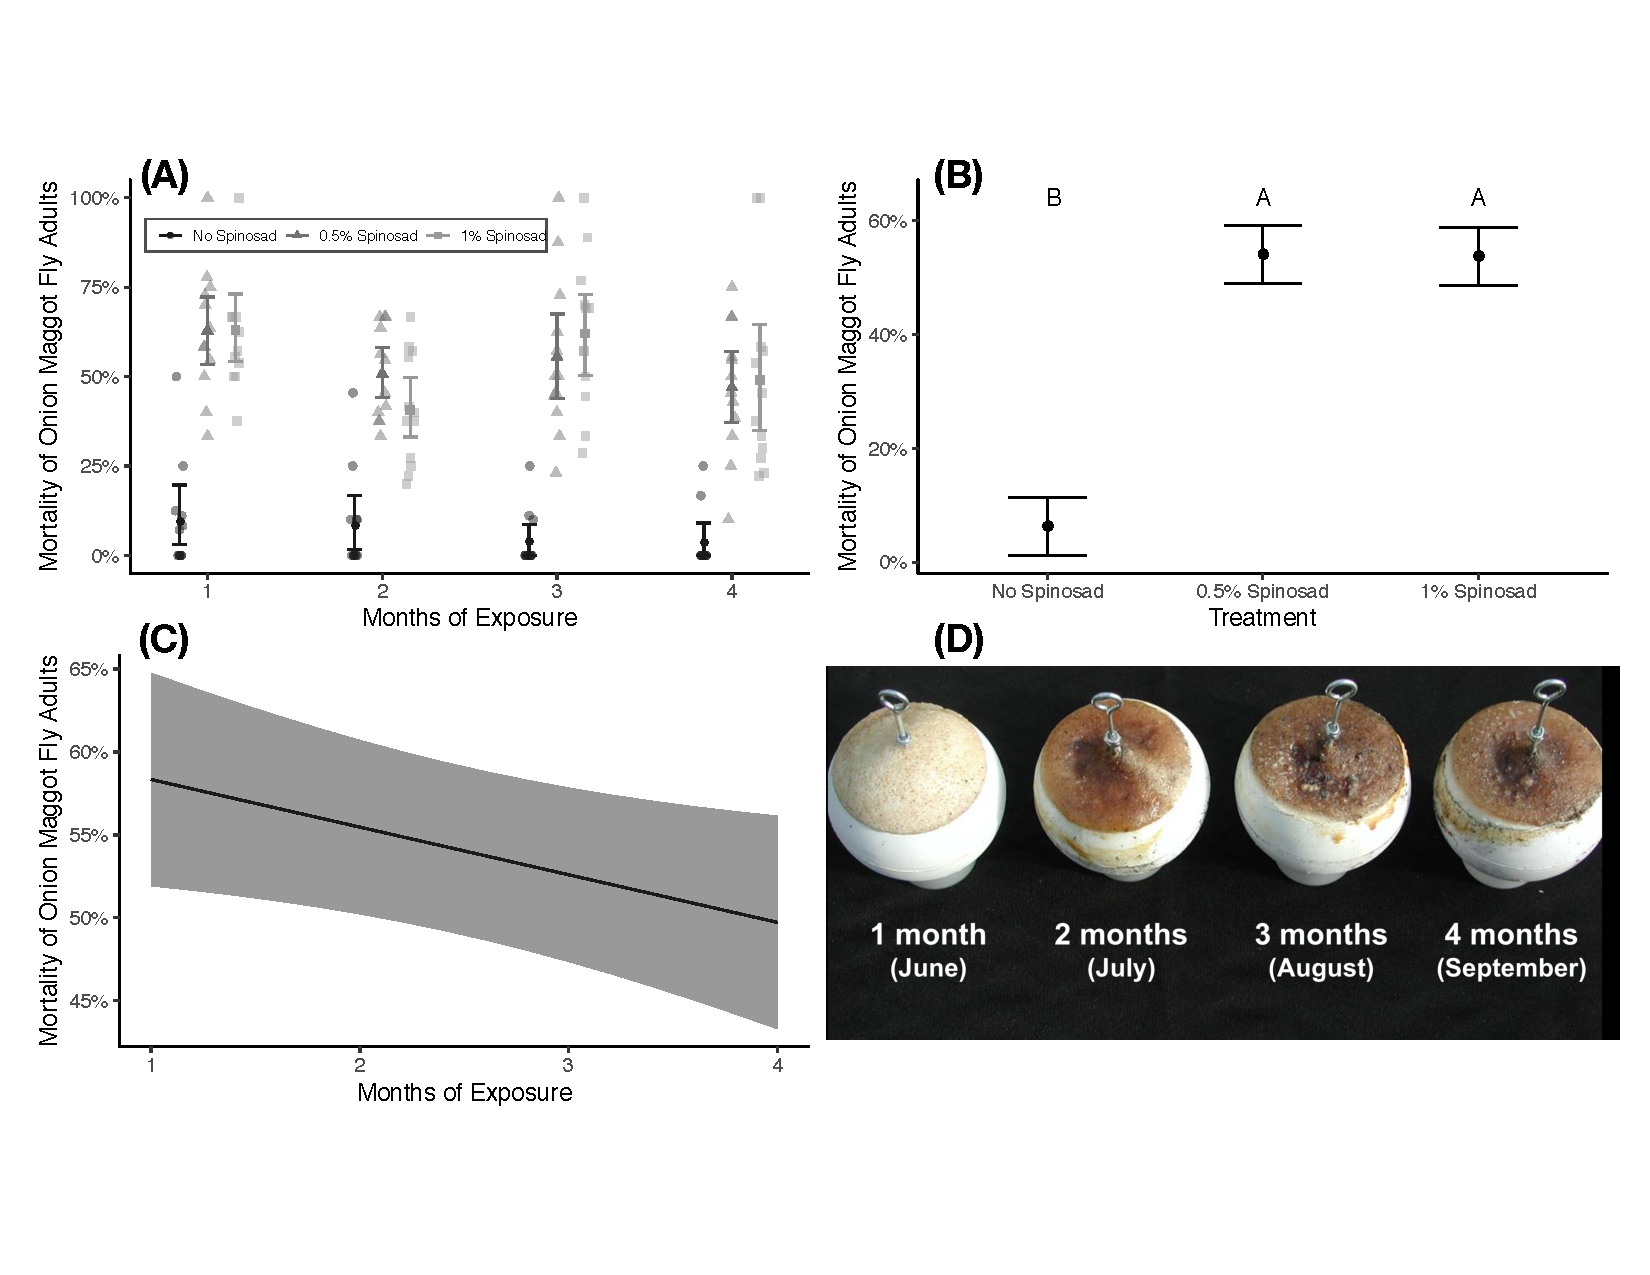
\includegraphics[width = 8cm]{figures/final-figures/figure-2.pdf}
\caption{Adult onion maggot (\textit{D. antiqua} mortality in the presence of spinosad treated spheres.  (A) Raw data of effects of exposure time and spinosad rate on mortality of adult onion maggot flies.  Light points indicate individual observations.  Solid points and error bars denote mean and 95\% confidence intervals respectively.  (B) Main effects of spinosad rate on adult onion maggot mortality.  Points and error bars denote mean effect and 95\% confidence intervals respectively.  Different letters denote significant differences (p \textless 0.05).  (C) Main effect of exposure time on adult onion maggot mortality.  Line and shaded area denote effect and 95\% confidence region respectively.  (D) Photographs of spinosad treated spheres at increasing exposure time in field conditions.  Spheres were placed in the field on the 15th of May.  }
\label{fig:figure2}
\end{figure}


\begin{figure}[bt]
\centering
\includegraphics[width = 8cm]{figures/final-figures/figure-3.pdf}
\caption{Adult onion maggot fly mortality following introduction to cages containing spinosad treated spheres.  Spheres were treated with differing rates of spinosad (rows) and exposed to field conditions for increasing amounts of time (column).  Lines and shaded regions indicate fitted smoothed (LOESS) mortality rates and 95\% confidence regions respectivel.  }
\label{fig:figure3}
\end{figure}


\begin{figure}[bt]
\centering
\includegraphics[width = 8cm]{figures/final-figures/figure-4.pdf}
\caption{Field damage of onions.  (A) End of season stand loss of onions (number of dead onion plants) as a result of all mortality factors.  (B) Cumulative damage (number of dead onion plants) as a result of onion maggot larval feeding.  Light points indicate observed values.  Solid points and errorbars denote mean effects and 95\% confidence intevals respectively.  Different letters denote significant differences (p \textless 0.05).   }
\label{fig:figure4}
\end{figure}


\begin{figure}[bt]
\centering
\includegraphics[width = 8cm]{figures/final-figures/figure-5.pdf}
\caption{Field damage of onion in enclosed cages with differing spinosad sphere formulations.  Cumulative damage is number of dead plants as a result of onion maggot damage.  Points and error bars denote mean and 95\% confidence intervals respectively.  Different letters denote significant differences (p \textless 0.05).  }
\label{fig:figure4}
\end{figure}





\section{Discussion}


\section*{Acknowledgements}
Suggestions for acknowledgements?

\section*{Conflict of Interest}
The authors declare no conflict of interest.  

\section*{Author Contribution}
BAN, JPN, and SW designed the experiments.  DSW, CCF, and BAN analyzed the data and wrote the manuscript.  


\section*{Data Availability Statement}
All code and data, including manuscript documentation, is available on GitHub(https://github.com/acetworld/onion-maggot-attraction).

%\printendnotes


\section{References}

\bibliographystyle{vancouver-authoryear}
\bibliography{om-attraction}

\graphicalabstract{example-image-1x1}{Please check the journal's author guildines for whether a graphical abstract, key points, new findings, or other items are required for display in the Table of Contents.}

\end{document}
